%==============================================================================
% presentation.tex
%==============================================================================


%==============================================================================
% Configuration
%==============================================================================

% Internationalisation
\usepackage[utf8]{inputenc}
\usepackage[T1]{fontenc}
% \usepackage[ngerman]{babel}

% Different packages
\usepackage{url}
\usepackage{color,listings,paralist}
\usepackage{enumerate}
\usepackage{tabularx}
\usepackage{alltt}

% Use default Acrobat reader fonts
\usepackage{mathpazo}

% Use CM fonts (increases document size)
\usepackage{ae}

% Use images
\usepackage{graphicx}

% Configure beamer
\usetheme[secheader]{Ikhono}
\usefonttheme[onlylarge]{structurebold}
\setbeamertemplate{navigation symbols}{}

% Variables
\providecommand{\Title}{Mining Software Repositories for Intelligent
  Software Maintenance}
\providecommand{\ShortTitle}{Mining software repositories}
\providecommand{\Author}{Thomas Weibel <weibelt@ethz.ch>}
\providecommand{\Institute}{SETLabs, Infosys Tech. Ltd., Bangalore}
\providecommand{\Date}{December 1, 2009}

% PDF settings
\hypersetup{
  pdftitle={\Title},
  pdfauthor={\Author},
  pdfsubject={\Institute},
  pdfkeywords={software engineering, portable, efficient, parallel
    programming language} 
}

% Titlepage
\title[\ShortTitle]{\Title}
\author{\Author}
\institute{\Institute}
\date{\Date}

% Listings
\lstdefinelanguage[]{Metrics}[]{}{
  keywords={if,then,else,end}
}
\lstdefinestyle{Default}{
  language=Metrics,
  tabsize=2,
  mathescape=true,
  inputencoding=utf8,
  showstringspaces=false,
  fontadjust=true,
  basicstyle=\ttfamily,
  keywordstyle=\color{blue}\bfseries,
}
\lstset{style=Default}


%==============================================================================
% Document
%==============================================================================

\begin{document}


% Titlepage
\begin{frame}[plain]
  \titlepage
\end{frame}

\note{
}


\section*{Introduction}

\begin{frame}{Executive Summary}
  \begin{itemize}
  \item Change management with version control systems
  \item Improving software maintenance through software repository
    mining
  \item Framework for preventive maintenance
  \item Novelty: Metrics for localization
  \item Study of Open Source projects
  \end{itemize}
\end{frame}

\note{
  \begin{itemize}
  \item First I will introduce change management with version control
    systems.
  \item Then I will show you how you can improve software maintenance
    through software repository mining
  \item After this, I'm going present you a framework for preventive
    maintenance I developed.
  \item As a novelty, we devised a metrics for localization.
  \item And did a study of Open Source projects.
  \end{itemize}
}


\section{Version Control}

\begin{frame}{Outline}
  \tableofcontents[current]
\end{frame}

\note{
}

\begin{frame}{Version Control}
  \begin{center}
    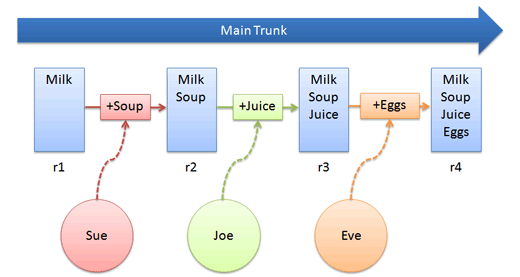
\includegraphics[scale=0.35]{figures/vcs}
  \end{center}

  \vspace{\stretch{1}}

  \begin{itemize}
  \item Management of changes to computer files in a repository
  \item Changes identified by a number or letter code (``revision'')
  \item Each revision associated with timestamp and person
    making the change
  \item Version control systems: CVS, Subversion, Git, ...
  \end{itemize}
\end{frame}

\note{
  \begin{itemize}
  \item Version control is the management of changes to documents,
    programs, and other information stored as computer files. It is
    most commonly used in software development, where a team of people
    may be changing the same files.
  \item Changes are usually identified by a number or letter code,
    termed the ``revision''. For example, an initial set of files is
    ``revision 1''. When the first change is made, the resulting set
    is ``revision 2'', and so on.
  \item Each revision is associated with a timestamp and the person
    making the change.
  \item Examples of version control systems are CVS, Subversion or
    Git.
  \end{itemize}
}

\begin{frame}[containsverbatim]{Working Copy, Commits and Change Sets}
  \begin{itemize}
  \item Working copy: Local copy of files from a repository
  \item Commit: Writing changes to the working copy into the
    repository
  \item Change set: Set of changes made in a single commit
  \end{itemize}

  \vspace{\stretch{1}}

\begin{verbatim}
  commit 3d2d827f5ca5e32816194119d5c980c7e04474a6
  Author: Michael S. Tsirkin <mst@redhat.com>
  Date:   Mon Sep 21 17:03:51 2009 -0700

      mm: move use_mm/unuse_mm from aio.c to mm/

  M       fs/aio.c
  A       include/linux/mmu_context.h
  M       mm/Makefile
  A       mm/mmu_context.c
\end{verbatim}
\end{frame}

\note{
  \begin{itemize}
  \item The working copy is the local copy of files from a repository,
    at a specific time or revision.
  \item A commit occurs when a copy of the changes made to the working
    copy is written or merged into the repository.
  \item On version control systems with atomic multi-change commits, a
    change set identifies the set of changes made in a single commit.
  \item Explain commit!
  \end{itemize}
}


\section{Mining Software Repositories}

\begin{frame}{Outline}
  \tableofcontents[current]
\end{frame}

\note{
}

\begin{frame}{Software Repository Mining}
  \begin{columns}[c]
    \begin{column}{0.60\textwidth}
      \begin{itemize}
      \item Version control systems contain large amounts of
        historical information: ``\textit{Who} changed \textit{what},
        \textit{why} and \textit{when}.''
      \item Learn from the past to shape the future
      \item Automated extraction, collection, and abstraction of
        information from software development data
      \end{itemize}
    \end{column}
    \begin{column}{0.40\textwidth}
      
\includegraphics[width=\textwidth]{figures/mining}
    \end{column}
  \end{columns}
\end{frame}

\note{ 
  \begin{itemize}
  \item Version control systems contain large amounts of historical
    information that can give deep insight into the evolution of a
    software project: ``\textit{Who} changed \textit{what},
    \textit{why} and \textit{when}.''
  \item When mining software archives, we want to learn from the past
    to shape the future.
  \item The mining of software repositories is concerned with the
    automated extraction, collection, and abstraction of information
    from available software development data.
  \end{itemize}
}

\begin{frame}{Populating Version History Database}
  \begin{center}
    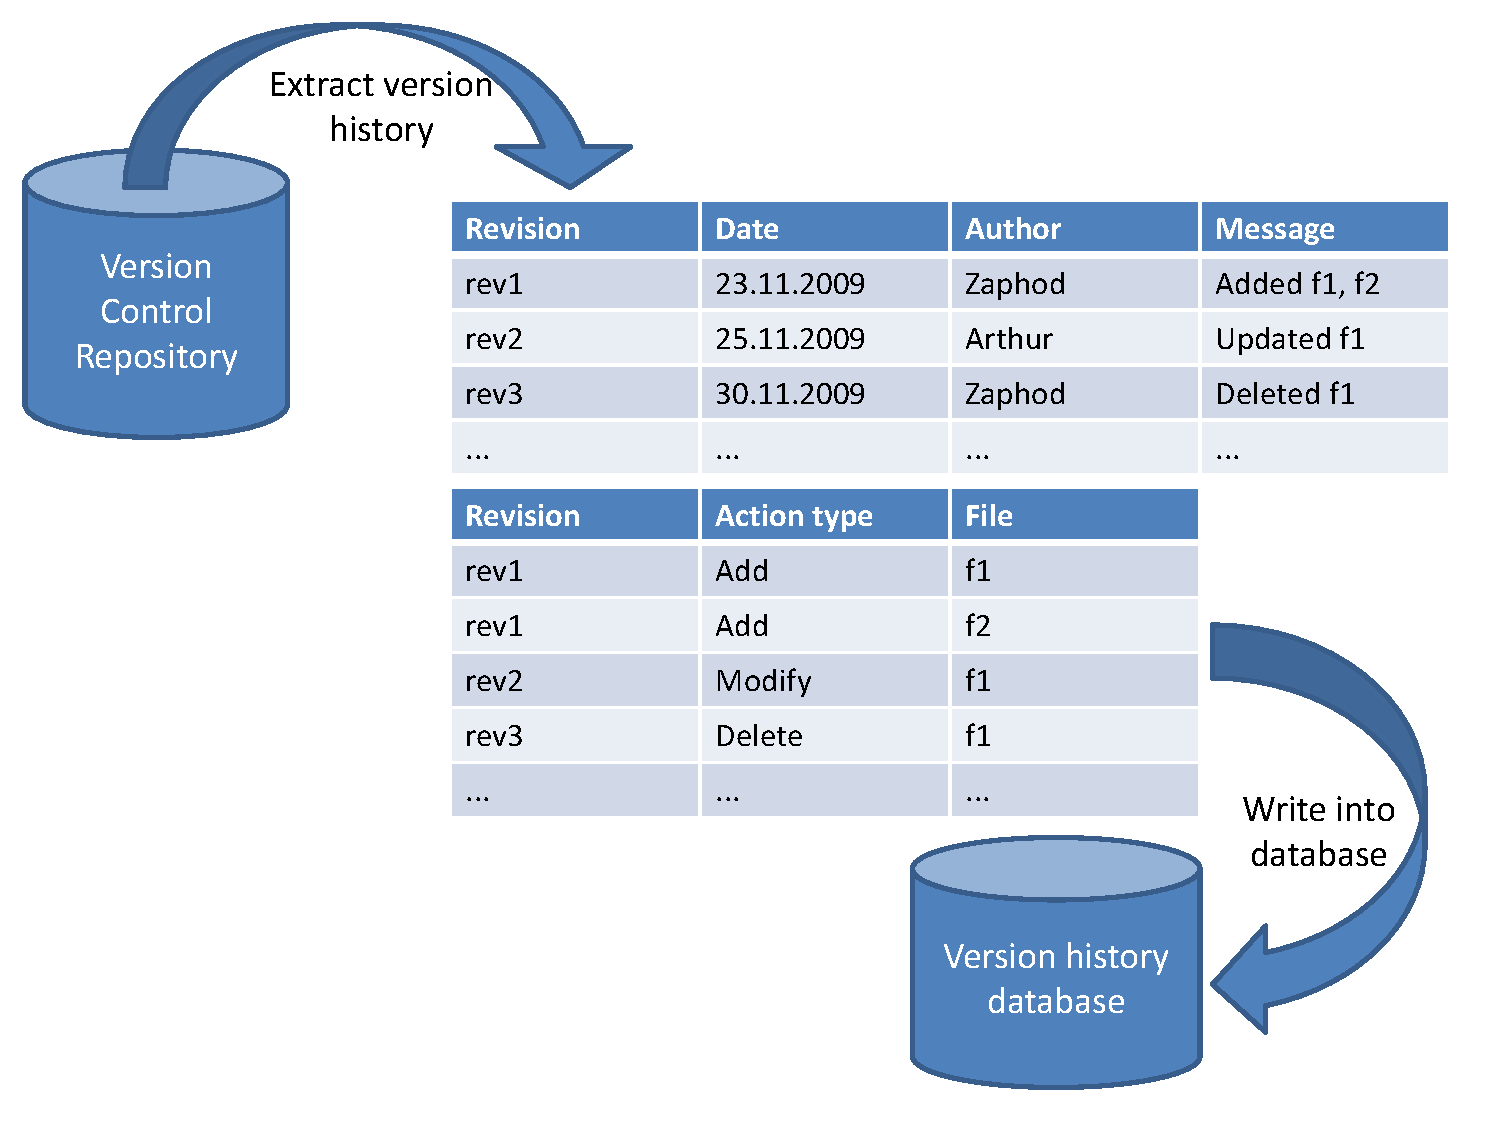
\includegraphics[width=0.95\textwidth]{figures/extracting-version-history}
  \end{center}
\end{frame}

\note{
  \begin{itemize}
  \item First we extract version history from the version control
    repository.
  \item This gives us information about who changes what, why and when.
  \item This information is written into a version history database
    for easier mining.
  \end{itemize}
}

\subsection{Frequent Item Set Mining}

\begin{frame}{Frequent Item Set Mining}
  \begin{columns}[c]
    \begin{column}{0.5\textwidth}
      \begin{itemize}
      \item Popular method for market basket analysis
      \item Identify sets of products frequently bought together: Beer
        and diapers
      \item Framework applies frequent item set mining to the version
        history of software repositories
      \item Identify which code files have been frequently changed
        together
      \end{itemize}
    \end{column}
    \begin{column}{0.5\textwidth}
      \begin{center}
        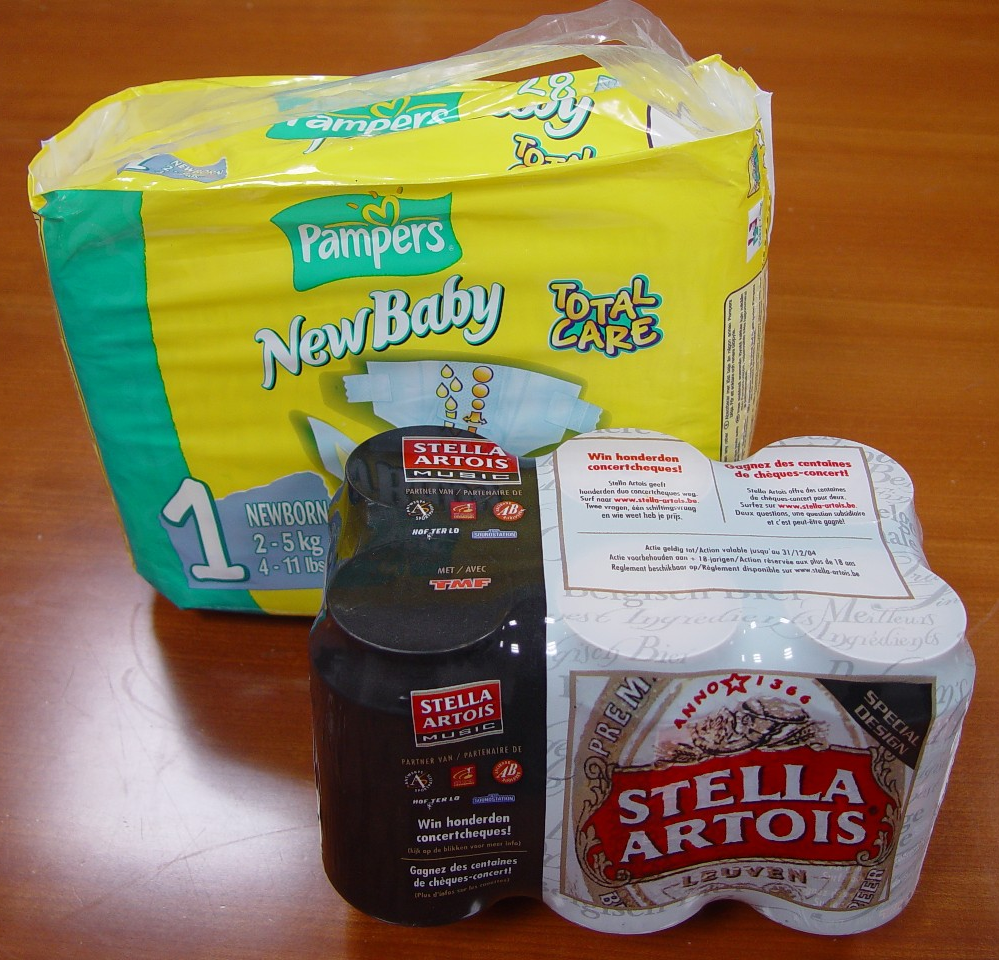
\includegraphics[width=\textwidth]{figures/frequent-item-set} \\
        \tiny{Source: \url{http://research.nii.ac.jp/~uno}}
      \end{center}
    \end{column}
  \end{columns}
\end{frame}

\note{
  \begin{itemize}
  \item Finding frequent item sets in a set of transactions is a
    popular method for so-called market basket analysis. It aims at
    finding regularities in the shopping behaviour of customers of
    supermarkets, mail-order companies, online-shops and so forth.
  \item In particular, it tries to identify sets of products that are
    frequently bought together:
  \item A famous example was the discovery that people who buy diapers
    also frequently buy beer. Those are probably exhausted fathers of
    small children.
  \item Therefore nowadays one finds frequently beer close to diapers
    - and of course also chips close to beer - in supermarkets.
  \item In our framework, we apply frequent item set mining to the
    version history of software repositories.
  \item The goal is to find out, which code files have been frequently
    changed together.
  \end{itemize}
}

\begin{frame}[containsverbatim]{Frequent Item Set Mining: Transactions}
  \begin{itemize}
  \item Transactions: Change sets
  \item Example:
\begin{verbatim}
  { fs/aio.c, include/linux/mmu_context.h, 
    mm/Makefile, mm/mmu_context.c }
\end{verbatim}
  \end{itemize}

  \vspace{\stretch{1}}

\begin{verbatim}
  commit 3d2d827f5ca5e32816194119d5c980c7e04474a6

  M       fs/aio.c
  A       include/linux/mmu_context.h
  M       mm/Makefile
  A       mm/mmu_context.c
\end{verbatim}
\end{frame}

\note{
  \begin{itemize}
  \item A change set identifies the set of changes made in a single
    commit to the version control system. We take change sets as our
    transactions in frequent item set mining.
  \item In the example below, the transaction consist of four files.
  \end{itemize}
}

\begin{frame}{Frequent Item Set Mining: Definitions}
  \begin{itemize}
  \item \alert{Transaction database} contains all change sets
  \item Members of transactions are \alert{items}
  \item \alert{Item set} is a subset of possible items
  \item \alert{Support} of an item set $i$: sup($i$) $:=$ number of
    transactions $t$ that contain $i$
  \end{itemize}
\end{frame}

\note{
  \begin{itemize}
  \item The \alert{transaction database} contains all transactions of
    the version control system.
  \item Members of transactions are called \alert{items}.
  \item And and \alert{item set} is a subset of possible items
  \item The \alert{support} of an item set $i$ is the number of
    transactions $t$ that support - this means contain - $i$.
  \end{itemize}
}

\begin{frame}{Frequent Item Set Mining: Association Rules}
  \begin{center}
    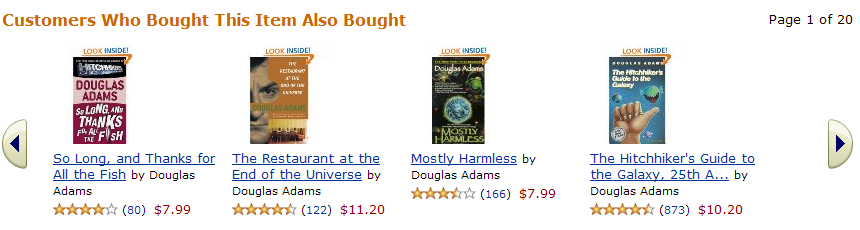
\includegraphics[width=\textwidth]{figures/frequent-items} \\
    \tiny{Source: \url{amazon.com}}
  \end{center}

  \vspace{\stretch{1}}

  \begin{itemize}
  \item \alert{If} a customer buys \alert{bread} and \alert{wine}, \\
    \alert{then} she will probably also buy \alert{cheese}
  \item Problem decomposed into two subproblems:
    \begin{itemize}
    \item Finding frequent item sets with minimum support
    \item Generate association rules with minimal confidence
    \end{itemize}
  \item Confidence for association rule $R: X \rightarrow Y$:
    $\text{conf}(R) = \text{conf}(X \rightarrow Y) =
    \text{sup}(X \cup Y)/\text{sup}(X)$
  \end{itemize}
\end{frame}

\note{
  \begin{itemize}
  \item Association rule mining gives options to finish the sentence
    ``Customers who bought this item also bought...''
  \item For example ``\alert{If} a customer buys \alert{bread} and
    \alert{wine}, \alert{then} she will probably also buy
    \alert{cheese}''.
  \item The problem is decomposed into two subproblems:
    \begin{itemize}
    \item Finding frequent item sets with minimum support
    \item Generate association rules with minimal confidence
    \end{itemize}
  \item Instead of going into details about confidences, I will give
    you an example for frequent item set mining and association rules.
  \end{itemize}
}

\begin{frame}{Frequent Item Set Mining: Example}
  \begin{center}
    \begin{tabular}{c|l}
      Transaction IDs & Transactions (Files) \\ \hline \hline
      1 & $\{1, 2, 3, 4\}$ \\ \hline
      2 & $\{2, 3, 4\}$ \\ \hline
      3 & $\{2, 3\}$ \\ \hline
      4 & $\{1, 2, 4\}$ \\ \hline
      5 & $\{1, 2, 3, 4\}$ \\ \hline
      6 & $\{2, 4\}$ \\
    \end{tabular}
  \end{center}
\end{frame}

\note{
  Show example on the whiteboard
}

\subsection{Maintenance Challenges}

\begin{frame}{Maintenance Challenges}
  \begin{itemize}
  \item Predicting changes
    \begin{itemize}
    \item Incomplete changes
    \end{itemize}
  \item Traceability links
    \begin{itemize}
    \item ``Cross-language'' changes
    \end{itemize}
  \item Predicting faults
  \item Understanding software evolution
    \begin{itemize}
    \item Measure change localization
    \end{itemize}
  \end{itemize}

  \vspace{\stretch{1}}

  \begin{center}
    
\includegraphics[width=0.7\textwidth]{figures/dilbert-software-changes}
  \end{center}
\end{frame}

\note{
}

\begin{frame}{Predicting Changes}
  \begin{thebibliography}
    \beamertemplatearticlebibitems
  \bibitem{predicting-source-code-changes}
    A. Ying, G. Murphy et al., {\em Predicting Source Code Changes by
      Mining Change History}
  \end{thebibliography}

  \vspace{\stretch{1}}

  \begin{itemize}
  \item Determines change patterns from change history of the code
    base
  \item Uses association rule mining for identifying implicit
    dependencies
  \item Change patterns can be used to recommend potentially relevant
    source code to a developer performing a modification task
  \end{itemize}
\end{frame}

\note{
  \begin{itemize}
  \item Determines change patterns from the change history of the code
    base. Change patterns are sets of files that were changed together
    frequently in the past. This means, they are frequent item sets.
  \item The method uses association rule mining for identifying
    implicit dependencies
  \item Change patterns can be used to recommend potentially relevant
    source code to a developer performing a modification task
  \end{itemize}
}

\begin{frame}{Predicting Changes: Incomplete Change}
  \begin{itemize}
  \item Comments in modification task report of Mozilla:
    \begin{itemize}
    \item 2002-06-12 14:14: Patch to gtk/nsFontMetricsGTK.cpp,
      limiting the size of fonts to twice the display height.
    \item 2002-06-12 14:37: Patch misses the Xlib version.
    \item A patch was later submitted with the correct changes in the
      X-windows font handling code in the file
      xlib/nsFontMetricsXlib.cpp
    \end{itemize}
  \item gtk/nsFontMetricsGTK.cpp does not reference
    xlib/nsFontMetricsXlib.cpp $\rightarrow$ used in different
    configurations
  \item Files were changed 41 times together $\rightarrow$ change
    pattern
  \item Changing the gtk/nsFontMetricsGTK.cpp could trigger a
    recommendation for xlib/nsFontMetricsXlib.cpp
  \end{itemize}
\end{frame}

\note{
  \begin{itemize}
  \item The Mozilla Web browser includes a Web content layout engine
    responsible for Web pages. There was a bug that caused the
    consumption of all available memory when a Web page with very
    large fonts was displayed. The comments in the modification task
    report include the following:
    \begin{itemize}
    \item 2002-06-12 14:14: Patch to gtk/nsFontMetricsGTK.cpp,
      limiting the size of fonts to twice the display height.
    \item 2002-06-12 14:37: Patch misses the Xlib version.
    \item A patch was later submitted with the correct changes in the
      X-windows font handling code in the file
      xlib/nsFontMetricsXlib.cpp
    \end{itemize}
  \item The source code in gtk/nsFontMetricsGTK.cpp does not reference
    the code in xlib/nsFontMetricsXlib.cpp because the code in the gtk
    version and the code in xlib version are used in different
    configurations of Mozilla.
  \item However, an analysis of the change history for Mozilla
    indicates that these two files were changed 41 times together.
  \item When we applied our approach to Mozilla, we extracted a change
    pattern. Changing the gtk/nsFontMetricsGTK.cpp could trigger a
    recommendation for the other file.
  \end{itemize}
}

\begin{frame}{Traceability Links}
  \begin{thebibliography}
    \beamertemplatearticlebibitems
  \bibitem{traceability-links}
    H. Kadgi et al., {\em Mining Software Repositories for
      Traceability Link}
  \end{thebibliography}

  \vspace{\stretch{1}}

  \begin{itemize}
  \item If files of difference types are co-changed with a high
    frequency over multiple versions $\rightarrow$ potential
    traceability link
  \item Traceability links derived from the actual changes to files by
    mining software repositories
  \item Uses sequential-pattern mining to identify and analyze sets of
    files that are committed together
  \item Sequential-pattern mining produces ordered lists of
    co-changing files
  \item Ordering information can be used to infer directionality
  \end{itemize}
\end{frame}

\note{
  \begin{itemize}
  \item If files of different types are co-changed with a high
    frequency over multiple versions, then such files potentially
    have a traceability link between them
  \item Traceability links are derived from the actual changes to
    files by mining software repositories
  \item Uses sequential-pattern mining to identify and analyze sets of
    files that are committed together. Another approach would be
    frequent item set mining.
  \item Sequential-pattern mining produces ordered lists of
    co-changing files whereas frequent item set mining produces sets.
  \item The ordering information can be used to infer directionality
    of traceability links
  \end{itemize}
}

\begin{frame}[containsverbatim]{Traceability Links: Example}
  \begin{itemize}
  \item Mining change sets in the Wine repository
  \item Changes are tested:
    \begin{itemize}
    \item 
\begin{verbatim}
./dlls/gdiplus/graphicspath.c ->
./dlls/gdiplus/tests/graphicspath.c
\end{verbatim}
    \item 
\begin{verbatim}
./dlls/inetmib1/main.c ->
./dlls/inetmib1/tests/main.c
\end{verbatim}
    \end{itemize}
  \item Cross language changes:
    \begin{itemize}
    \item
\begin{verbatim}
./dlls/rpcrt4/tests/server.c ->
./dlls/rpcrt4/tests/server.idl
\end{verbatim}
    \item
\begin{verbatim}
./dlls/dxgi/dxgi_private.h ->
./include/wine/winedxgi.idl
\end{verbatim}
    \end{itemize}
  \end{itemize}
\end{frame}

\note{
  \begin{itemize}
  \item Mining change sets in the Wine repository
  \item Changes are tested
  \item Identifies cross language changes
  \end{itemize}
}

\begin{frame}{Predicting Faults}
  \begin{thebibliography}
    \beamertemplatearticlebibitems
  \bibitem{predicting-faults}
    S. Kim, T. Zimmermann et al., {\em Predicting Faults from Cached
      History}
  \end{thebibliography}

  \vspace{\stretch{1}}

  \begin{itemize}
  \item Assumption: faults do not occur in isolation, but rather in
    bursts of several related faults
  \item Identifying bug fixes by mining commit messages: Searching for
    keywords such as ``Fixed'' or ``Bug'' and references to bug
    reports like ``42''
  \item Cache locations that are likely to have faults
  \item By consulting the cache at the moment a fault is fixed, a
    developer can detect likely fault-prone locations
  \end{itemize}
\end{frame}

\note{
  \begin{itemize}
  \item The basic assumption is that faults do not occur in isolation,
    but rather in bursts of several related faults.
  \item Therefore, one can cache locations that are likely to have
    faults: starting from the location of a known (fixed) fault, cache
    the location itself, any locations changed together with the
    fault, recently added locations, and recently changed locations.
  \item By consulting the cache at the moment a fault is fixed, a
    developer can detect likely fault-prone locations. This is useful
    for prioritizing verification and validation resources on the most
    fault prone files or entities.
  \item Identifying bug fixes by mining change log messages: Searching
    for keywords such as ``Fixed'' or ``Bug'' and references to bug
    reports like ``42''
  \end{itemize}
}


\section{Framework}

\begin{frame}{Outline}
  \tableofcontents[current]
\end{frame}

\note{
}

\begin{frame}{Architecture}
  \begin{center}
    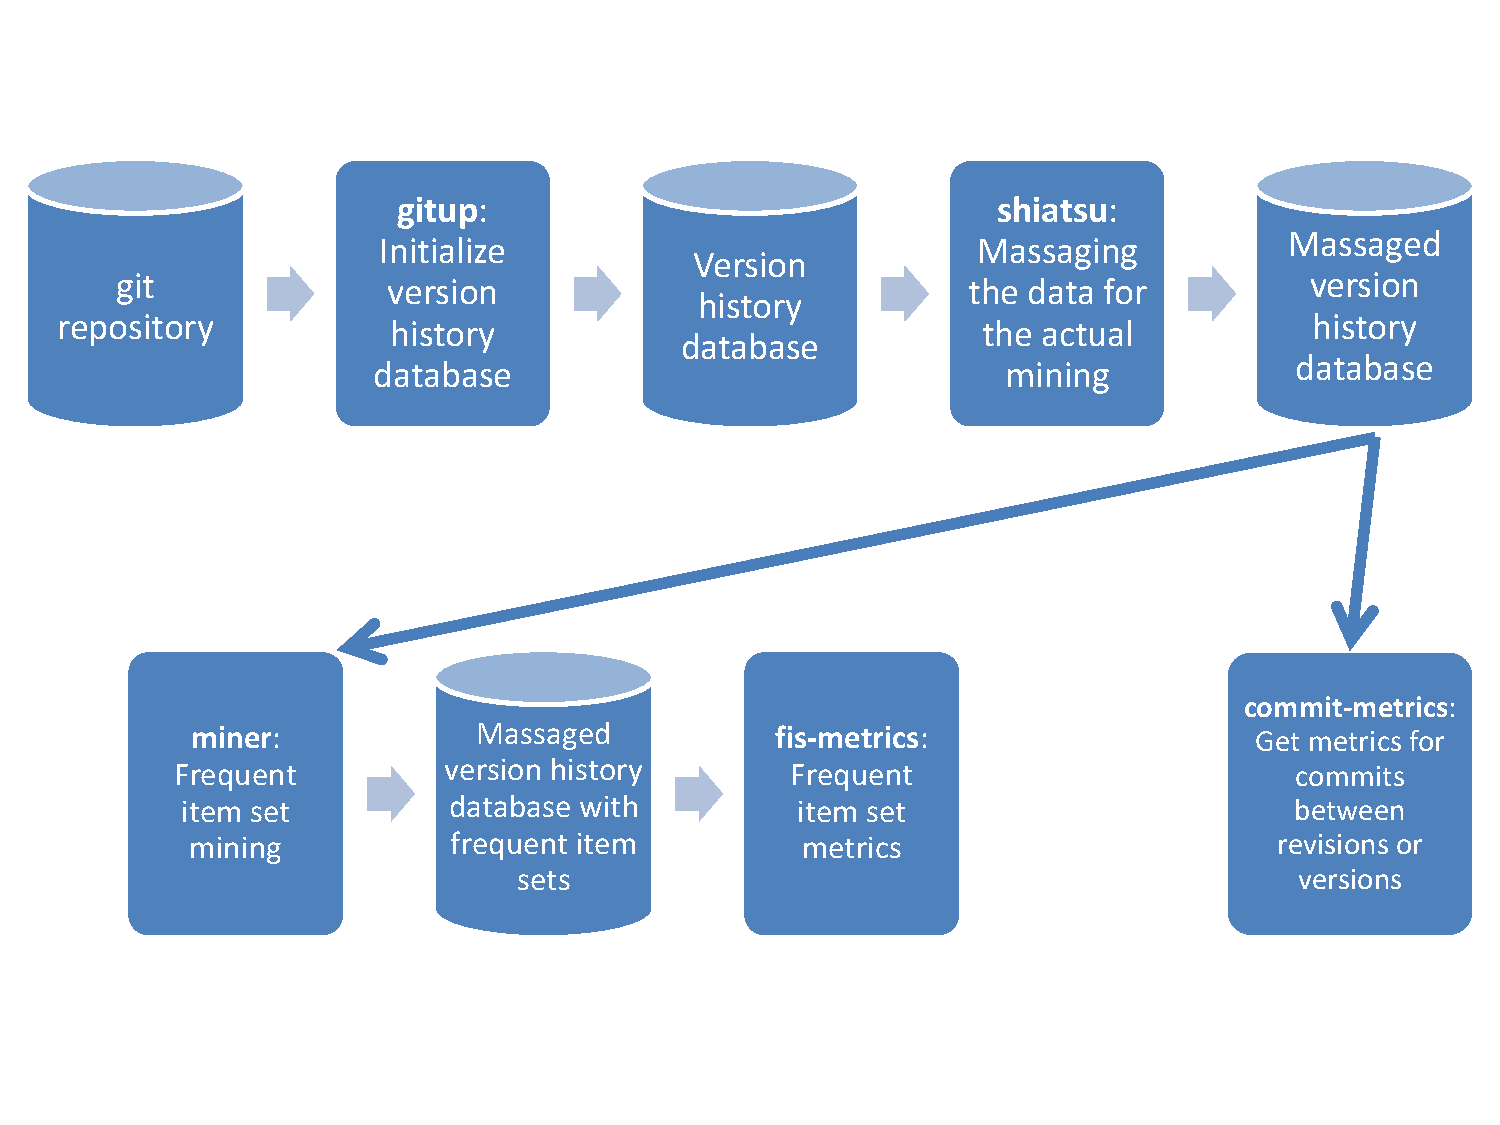
\includegraphics[width=0.95\textwidth]{figures/miner-architecture}
  \end{center}
\end{frame}

\note{
  \begin{itemize}
  \item We built a framework for software repository mining
  \item Explain framework!
  \end{itemize}
}

\begin{frame}{Git}
  \begin{itemize}
  \item Free distributed version control system
  \item Initially designed and developed for Linux kernel development
  \item Every working directory is a full-fledged repository:
    \begin{itemize}
    \item Complete history
    \item Full revision tracking capabilities
    \item Not dependent on network access or a central server
    \end{itemize}
  \item Easily convert repositories of other version control systems
    like Subversion into Git repositories
  \item Only need to write mining and analysis tools for one format
    rather than many
  \end{itemize}
\end{frame}

\note{
  \begin{itemize}
  \item We chose Git as the base of our framework.
  \item Git is a free distributed version control system.
  \item It was initially designed and developed by Linus Torvalds for
    Linux kernel development.
  \item Every Git working directory is a full-fledged repository with
    complete history and full revision tracking capabilities, not
    dependent on network access or a central server.
  \item Repositories of other version control systems like CVS or
    Subversion can easily be converted into Git repositories.
  \item This means we only need to write mining and analysis tools for
    one format rather than many.
  \end{itemize}
}

\begin{frame}{Populating the Version History Database}
  \begin{itemize}
  \item Gitup generates logfile and initializes versions history
    database
  \item Shiatsu massages the data to be used by the metrics
    applications
    \begin{itemize}
    \item Set modularization according to specified directory depth
    \item Remove deleted files
    \item Set number of modifications
    \item Heuristics for file moves
    \end{itemize}
  \item Massaged version history database is used to generate frequent
    item sets and calculate metrics
  \end{itemize}

  \vspace{\stretch{1}}

  \begin{center}
    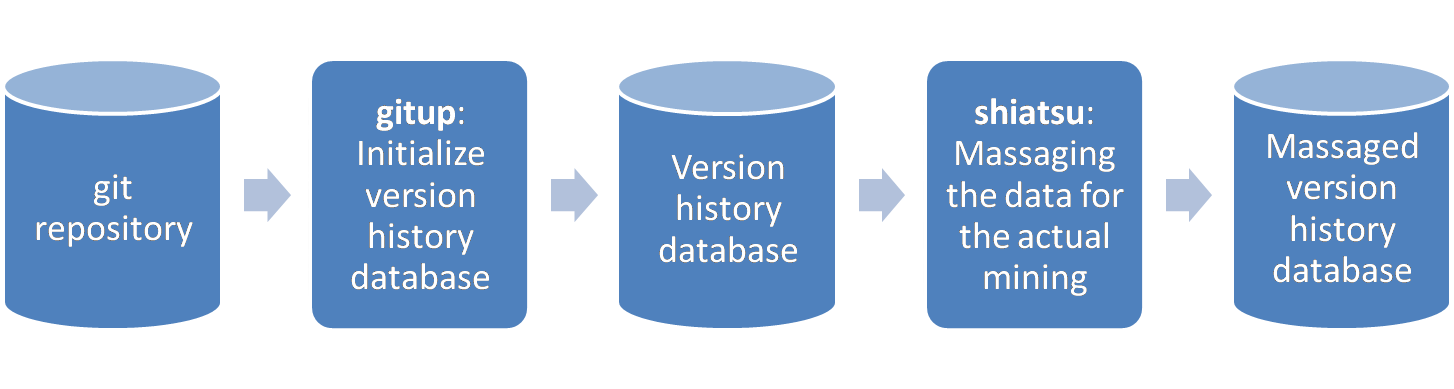
\includegraphics[width=0.95\textwidth]{figures/initialize-database}
  \end{center}
\end{frame}

\note{
  \begin{itemize}
  \item Gitup generates logfile and initializes versions history
    database.
  \item Shiatsu massages the data:
    \begin{itemize}
    \item It sets modularization according to specified directory depth.
    \item Shiatsu removes deleted files from the database and set the
      number of modifications.
    \item It also uses heuristics for file moves.
    \end{itemize}
  \item The massaged version history database is then used to generate
    frequent item sets and calculate metrics.
  \end{itemize}
}

\begin{frame}{Preventing Maintenance}
  Our framework can help with solving all mentioned maintenance
  challenges:

  \begin{itemize}
  \item Predicting changes
    \begin{itemize}
    \item Incomplete changes
    \end{itemize}
  \item Traceability links
    \begin{itemize}
    \item ``Cross-language'' changes
    \end{itemize}
  \item Predicting faults
  \item Understanding software evolution
    \begin{itemize}
    \item Measure change localization
    \end{itemize}
  \end{itemize}
\end{frame}

\note{
  Our framework can help with solving all mentioned maintenance
  challenges 
}


\section{Novelty}

\begin{frame}{Outline}
  \tableofcontents[current]
\end{frame}

\note{
}

\begin{frame}{Change Localization}
  \begin{itemize}
  \item A change is well localized, if it touches only one or very few
    modules
  \item A change is not well localized, if it touches many modules
  \item Apply change localization for frequent item sets
  \end{itemize}

  \vspace{\stretch{1}}

  \begin{block}{Hypothesis}
    Changes in frequent item sets in well modularized software systems
    are localized
  \end{block}
\end{frame}

\note{
  \begin{itemize}
  \item A change is well localized, if it touches only one or very few
    modules
  \item A change is not well localized, if it touches many modules
  \item Apply change localization for frequent item sets
  \item Our hypothesis is that changes in frequent item sets in well
    modularized software systems are localized
  \item This means that frequent item sets have a high localization
  \end{itemize}
}

\begin{frame}[containsverbatim]{Change Localization: Example}
  \begin{itemize}
  \item Well localized: Touches only one module
\begin{verbatim}
  dlls/ntdll/signal_i386.c
  dlls/ntdll/thread.c
\end{verbatim}
  \item Badly localized: Touches four modules out of five possible
\begin{verbatim}
  if1632/thunk.c
  include/process.h
  loader/task.c
  scheduler/process.c
  scheduler/thread.c
\end{verbatim}
  \item Not localized at all: Touches all possible modules
\begin{verbatim}
  files/dos_fs.c
  scheduler/syslevel.c
  tools/winapi-check  
\end{verbatim}
  \end{itemize}
\end{frame}

\note{
  Do the calculation after the next slide!

  \begin{itemize}
  \item $1 - 0 = 1$
  \item $1 - \frac{4}{5} = \frac{1}{5}$
  \item $1 - \frac{3}{3} = 1 - 1 = 0$
  \end{itemize}
}

\begin{frame}{Change Localization Metrics}
  \begin{itemize}
  \item Value between $0$ and $1$
  \item $0$: Not localized at all
  \item $1$: Fully localized
  \end{itemize}

  \vspace{\stretch{1}}

  \[
  \underline{\sum_{i = \text{FIS}_1}^{\text{FIS}_n} 1 -
    \left(\text{if}\left( i.\text{modules\_touched} = 1, 0,
        \frac{i.\text{modules\_touched}}{i.\text{files\_touched}}
      \right) \right)}
  \]
  \[
  n
  \]
\end{frame}

\note{
  Go back to the previous slide to show localization!
}


\section{Experiments}

\begin{frame}{Outline}
  \tableofcontents[current]
\end{frame}

\note{
}

\subsection{Linux 2.6}

\begin{frame}{Linux 2.6}
  \begin{columns}[c]
    \begin{column}{0.60\textwidth}
      \begin{itemize}
      \item Unix-like operating system kernel
      \item Repository checked out on November 19, 2009
      \item $25,277$ code files
      \item $168,800$ commits
      \item Frequent item set mining:
        \begin{itemize}
        \item Minimum number of commits (modifications) for code
          files: $4$
        \item Minimum support: $4$
        \item Maximum size of commits (number of code files): $50$
        \end{itemize}
      \end{itemize}
    \end{column}
    \begin{column}{0.40\textwidth}
      
\includegraphics[width=\textwidth]{figures/linux-logo}
    \end{column}
  \end{columns}
\end{frame}

\note{
  \begin{itemize}
  \item Linux is a Unix-like operating system kernel.
  \item I checked out the repository of the mainline on November 19,
    2009
  \item It has $25,277$ code files and consists of $168,800$ commits
  \item Settings used for the frequent item set mining are:
    \begin{itemize}
    \item Minimum number of commits (modifications) a code file has to
      have to be added to the transactions file: $4$
    \item Minimum support: $4$
    \item Maximum size of commits (number of code files): $50$
    \end{itemize}
  \end{itemize}
}

\begin{frame}{Linux 2.6: Frequent Item Set Metrics}
  \begin{center}
    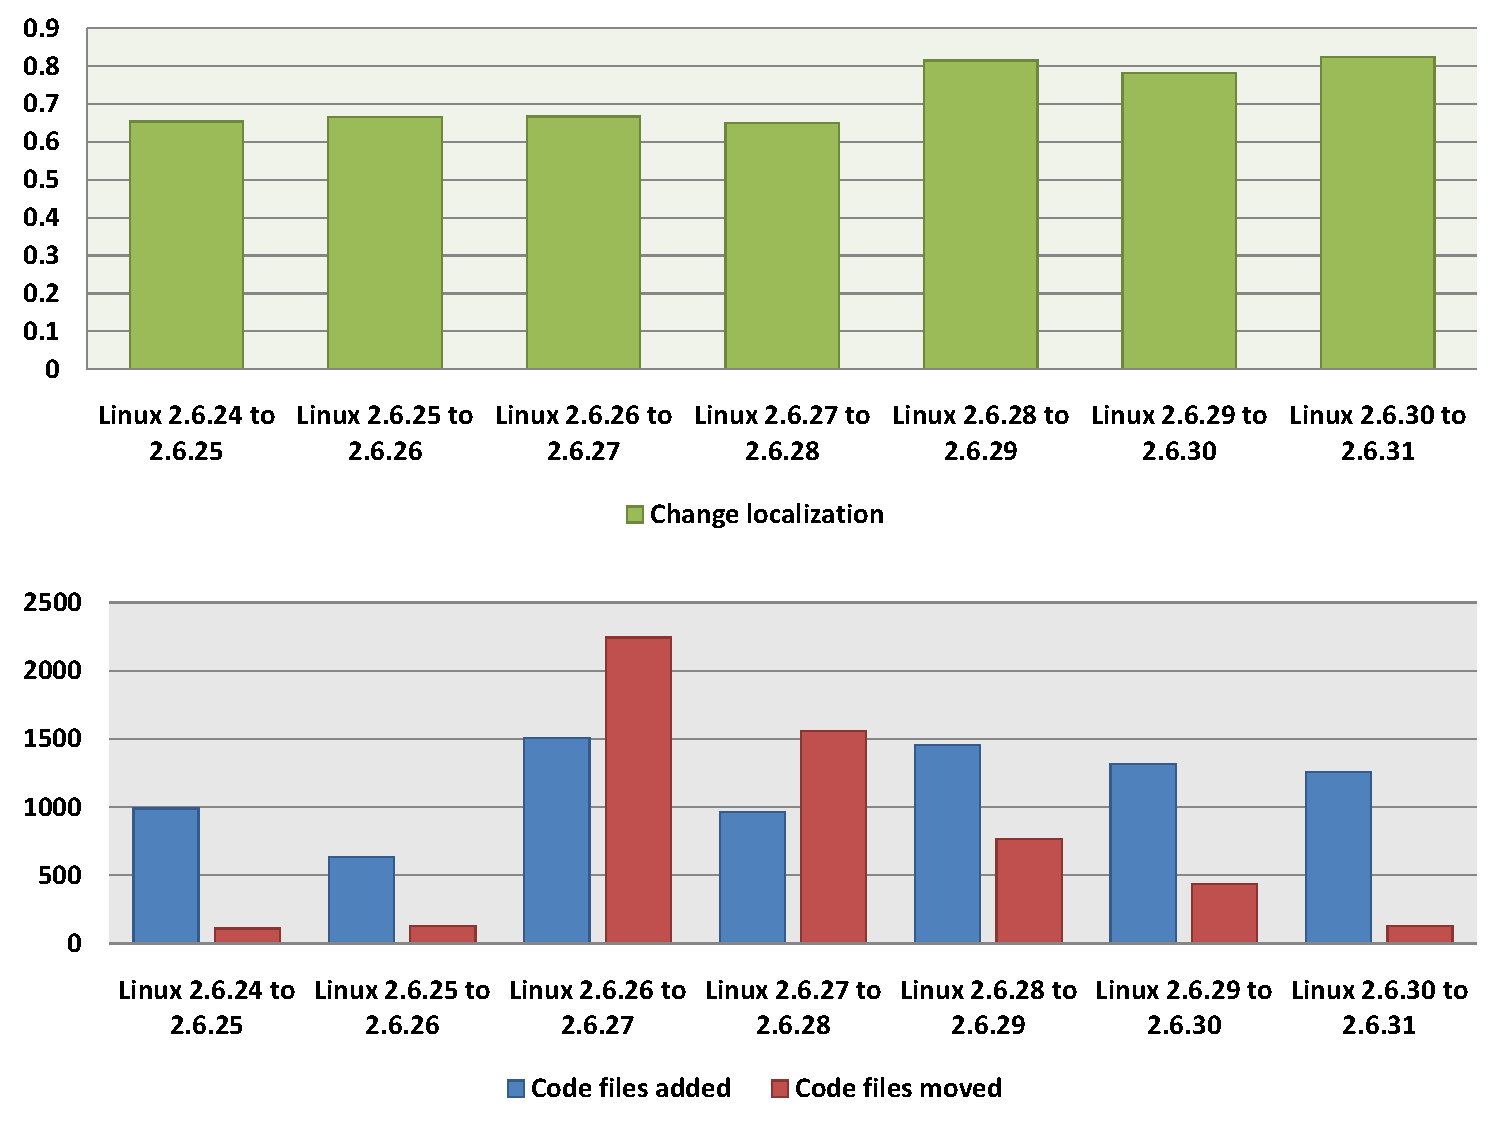
\includegraphics[width=0.95\textwidth]{minings/linux-2-6-fis-metrics}
  \end{center}
\end{frame}

\note{
  Explain how data was gathered: Log between tags (versions) in the
  repository.
}

\subsection{Wine}

\begin{frame}{Wine}
  \begin{columns}[c]
    \begin{column}{0.70\textwidth}
      \begin{itemize}
      \item Allows execution of Microsoft Windows programs on
        Unix-like operating systems
      \item Repository checked out on November 20, 2009
      \item $3,479$ code files
      \item $63,864$ commits
      \item Frequent item set mining:
        \begin{itemize}
        \item Minimum number of commits (modifications) for code
          files: $4$
        \item Minimum support: $4$
        \item Maximum size of commits (number of code files): $50$
        \end{itemize}
      \end{itemize}
    \end{column}
    \begin{column}{0.30\textwidth}
      
\includegraphics[width=\textwidth]{figures/wine-logo}
    \end{column}
  \end{columns}
\end{frame}

\note{
  \begin{itemize}
  \item Wine allows execution of Microsoft Windows programs on
    Unix-like operating systems
  \item I checked out the repository on November 20, 2009
  \item It has $3,479$ code files and consists of $63,864$ commits
  \item We use the same settings for the frequent item set mining as
    with Linux 2.6
  \end{itemize}
}

\begin{frame}{Wine: Frequent Item Set Metrics}
  \begin{center}
    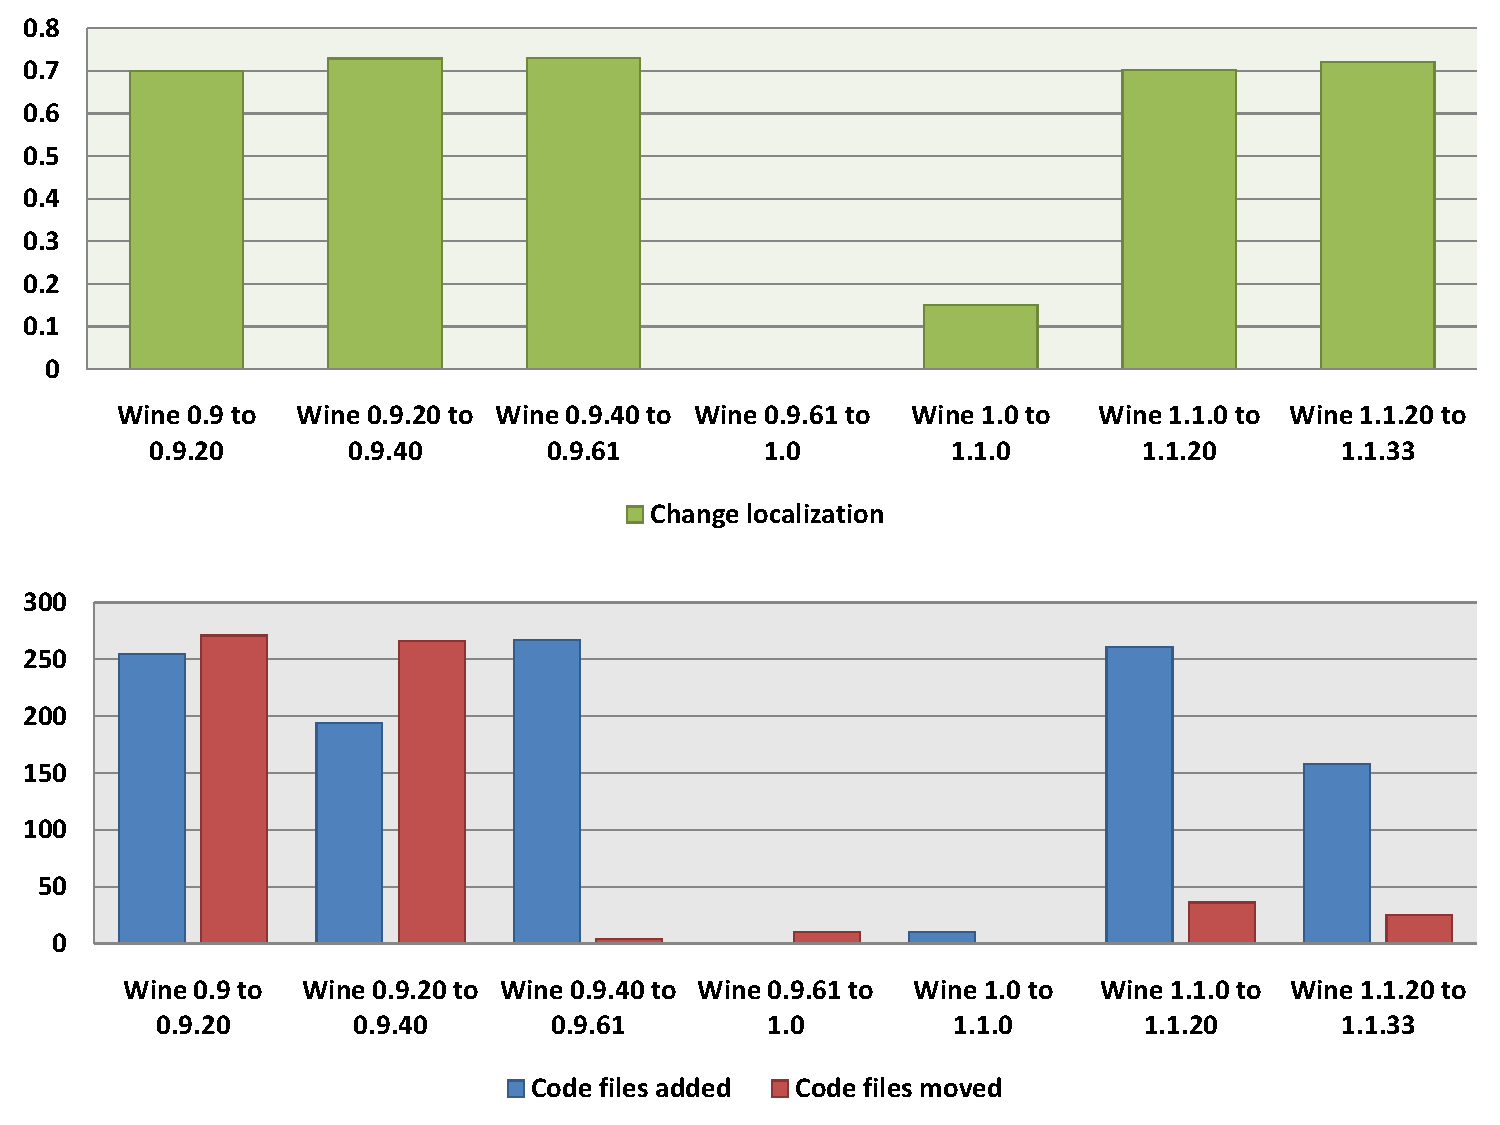
\includegraphics[width=0.95\textwidth]{minings/wine-fis-metrics}
  \end{center}
\end{frame}

\note{
}

\subsection{Insights}

\begin{frame}{Insights}
  \begin{itemize}
  \item Code file moves increase localization
  \item Adding of many code files decrease localization
  \item Adding of code files can clear effect of moves on localization
  \item Stable versions contain mostly bug fixes \\
    $\text{ }\Rightarrow$ low localization, only few moves and adds
  \item Unstable versions contain mostly new features \\
    $\text{ }\Rightarrow$ high localization, many moves and adds
  \end{itemize}
\end{frame}

\note{
  \begin{itemize}
  \item We got the following insights by examining Open Source
    software repositories:
  \item Code file moves increase localization
  \item Adding of many code files decrease localization
  \item Adding of code files can clear effect of moves on localization
  \item Stable versions contain mostly bug fixes \\
    this means they have a low localization and only few moves and
    adds
  \item Unstable versions contain mostly new features \\
    this means they have a high localization and many moves and adds
  \end{itemize}
}


\section*{Outro}

\begin{frame}{Future Work}
  \begin{itemize}
  \item Use framework to mine software repositories of commercial
    systems
  \item Compare localization metrics of Open Source and Closed Source
    systems
  \item Use the frequent item sets extracted to come up with a better
    modularization
  \item Publish research in the form of a paper
  \end{itemize}
\end{frame}

\note{
  \begin{itemize}
  \item We want to use our framework to mine software repositories of
    commercial systems.
  \item This would allow us to compare localization metrics of Open
    Source and Closed Source systems.
  \item Now after we introduced a way to measure change localization,
    we want to use the frequent item sets extracted from the version
    history to come up with a better modularization.
  \item Another goal is to publish the result of our research in the
    form of a paper.
  \end{itemize}
}

\begin{frame}{Summary}
  \begin{itemize}
  \item Mining software repositories for intelligent
    software maintenance
  \item Applications of frequent item set mining in improving software
    maintainability
  \item Framework for preventing software maintenance
  \item New metrics for change localization
  \item Localization of frequent item sets of Open Source projects
  \end{itemize}

  \vspace{\stretch{1}}

  \begin{center}
    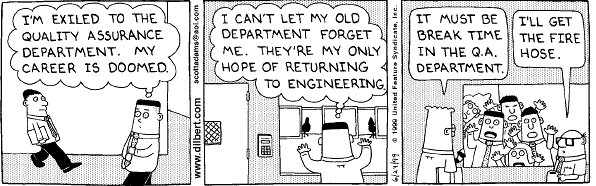
\includegraphics[width=0.7\textwidth]{figures/dilbert-quality-assurance}
  \end{center}
\end{frame}

\note{
  \begin{itemize}
  \item I presented mining software repositories for intelligent
    software maintenance.
  \item And have shown applications of frequent item set mining in
    improving software maintainability.
  \item I implemented framework for preventing software maintenance.
  \item And we Introduced new metrics for change localization.
  \item We used our framework and metrics to measure and analyze
    localization of frequent item sets of Open Source projects.
  \end{itemize}
}

\end{document}
